\documentclass[10pt]{article}
\usepackage[utf8]{inputenc}
\usepackage{hyperref}
\usepackage{fontenc}
\usepackage{mathptmx}
\usepackage{geometry}
\usepackage{titling}
\usepackage{graphicx}
\usepackage{subcaption}
\setlength{\topskip}{0mm}
\setlength{\droptitle}{-8em} 
\title{{\large \textbf{CONCORDIA UNIVERSITY \\ DEPARTMENT OF COMPUTER SCIENCE AND SOFTWARE ENGINEERING \\ SOEN 6011: SOFTWARE ENGINEERING PROCESSES \\ SECTION CC WINTER 2019 \\ F1: $arccos(x)$}  \\ }}
\author{\normalsize \textbf {STUDENT NAME: YONGCONG LEI} \\ \normalsize \textbf{STUDENT IDENTIFICATION NUMBER: 40045701 }}
\date{}
\begin{document}
\maketitle

\section{Characteristics and Domain}
\subsection{Characteristics}

\begin{enumerate}
    \item $arccos(x)$ is an inverse trigonometric functions of $cos(x)$. In order introduce inverse trigonometric functions, we first need to take a look at trigonometric functions. In mathematics, the trigonometric functions are real functions which relate an angle of a right-angled triangle to ratios of two side lengths\cite{einstein}. $cos(x)$ is one of them. Given $$x = cos(y) = \frac{b}{h} = \frac{adjacent}{hypotenuse}$$ then $$y = arccos(x)$$ Figure 1 is an example of $cos(x)$. In this case, $x = cos(y) = \frac{OC}{OA}$. Therefore, $y = arccos(x) = arccos(\frac{OC}{OA})$.
    \begin{center}
      \begin{figure}[h!]
          \centering
          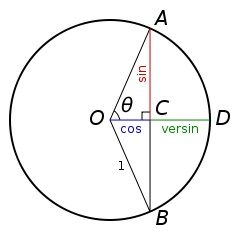
\includegraphics[width=0.3\linewidth]{image/cos_detail.jpg}
          \caption{trigonometric functions}
          \label{fig:my_label}
      \end{figure}
    \end{center}
    
    % \item principle values
    % \item relationship with $cos(x)$
    % \item $arccos(x)$ is a trigonometric function (relate an angle of a right-angled triangle to ratios of two side lengths).
    % \item 
\end{enumerate}

\subsection{Domain and Co-domain}
\paragraph{}
Since none of the six trigonometric functions are one-to-one, they are restricted in order to have inverse functions. As a result, we make a restriction here to restrict the co-domain of $arccos(x)$ in area $[0, \pi]$. Therefore, there will be one-to-one relationship between its domain and co-domain.

\paragraph{}
As a result, the domain is $x \in [-1, 1]$. The co-domain is $y \in [0, \pi]$ for the equation $y = arccos(x)$.

\begin{figure}
  \centering
  \begin{subfigure}[b]{0.4\linewidth}
    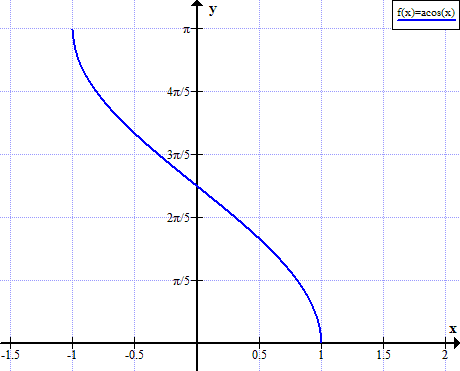
\includegraphics[width=\linewidth]{image/arccos.png}
    \caption{$arccos(x)$}
  \end{subfigure}
  \begin{subfigure}[b]{0.4\linewidth}
    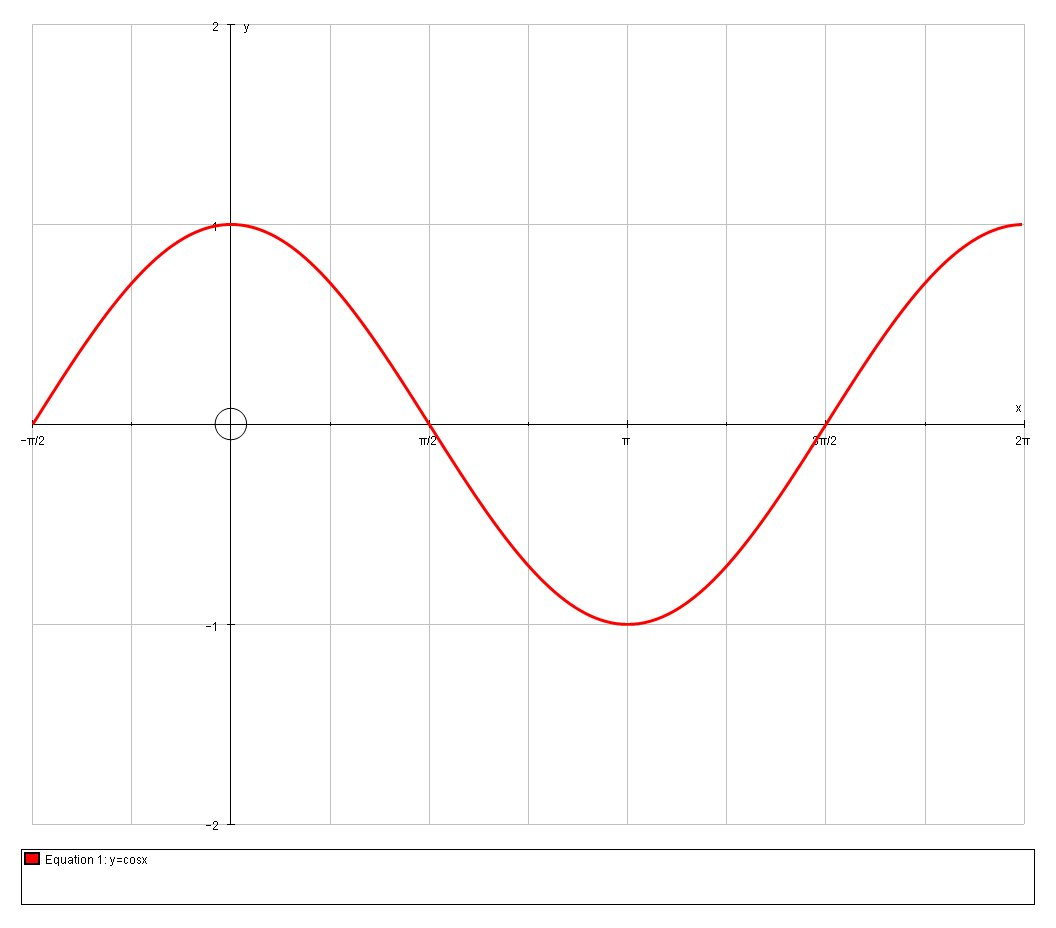
\includegraphics[width=\linewidth]{image/cos.jpg}
    \caption{$cos(x)$}
  \end{subfigure}
  \caption{$arccos(x)$ and $cos(x)$}
  \label{fig:coffee}
\end{figure}


\section{Requirements}

\section{Advantages and Disadvantages}

\section{References}
 
\end{document}
